\documentclass[12pt]{article}

\usepackage[bottom = 15mm]{geometry}
\usepackage[utf8]{inputenc}
\usepackage[T2A]{fontenc}
\usepackage[russian]{babel}
\usepackage{graphicx}
\usepackage{caption}
\usepackage{amssymb, gensymb, amsmath}
\usepackage{mathrsfs}
\usepackage{array, colortbl}


\textwidth = 16 cm
\textheight = 23  cm
\oddsidemargin = 0 pt
\topmargin = -1.5 cm
\parindent = 20 pt
\parskip = 0 pt
\flushbottom


\title{{\bf Задача 3.\,4.\,4 \\ Петля гистерезиса (статический метод)}}
\author{Лось Денис (группа 611)}
\date{19 октября 2017}




\begin{document}

\maketitle

\paragraph{Цель работы:} исследование кривых намагничивания ферромагнетиков с помощью баллистического гальванометра.

\paragraph{В работе используются:} генератор тока с источником питания, тороид, соленоид, баллистический гальванометр с осветителем и шкалой, мультиметр -- амперметр, лабораторный автотрансформатор, разделительный трансформатор.

\section*{Экспериментальная установка}
	Схема установки для исследования петли гистерезиса представлена на рис.1. К источнику постоянного напряжения подключён специальный генератор, позволяющий скачками менять токи в намагничивающей обмотке. Ток в намагничивающей обмотке измеряется цифровым мульметром $A$. Переключатель $P_1$ позволяет менять направление тока в первичной обмотке. Чувствительность гальванометра во вторичной цепи можно менять с помощью магазина сопротивлений $R_m$.
\begin{figure}[h!]
	\centering
	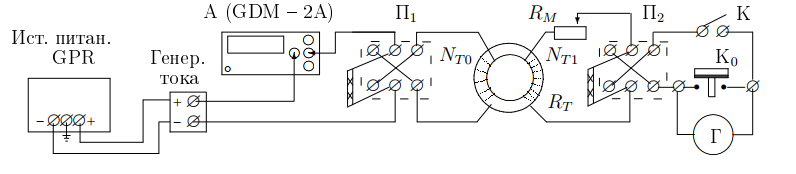
\includegraphics[height = 3cm, width = 12cm]{image1.png}
	\caption{Схема установки для исследования петли гистерезиса}
\end{figure}
\par
	Схема на рис.2 отличается от схемы на рис.1 только тем, что вместо тороида подключён калибровочный соленоид. Сопротивления измерительных цепей тороида ($R = R_T + R_M + R_0$) и соленоида ($R_1 = R_C + R_M' + R_0$) должны быть одинаковы. Сопротивление тороида $R_T \ll R_0$ --- сопротивления гальванометра, поэтому сопротивления магазина в схеме с тороидом и соленоидом отличаются на величину сопротивления соленоида $R_C$: $R_M' = R_M - R_C$.
\begin{figure}[h!]
	\centering
	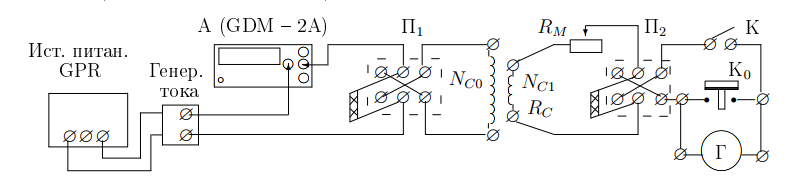
\includegraphics[height = 3cm, width = 12cm]{image2.png}
	\caption{Схема установки для калибровки гальванометра}
\end{figure}
\par
	Чтобы снять начальную кривую намагничивания, нужно размагнитить сердечник. Для этого тороид подключается к цепи переменного тока	(рис.3). При уменьшении амплитуды тока через намагничивающую обмотку от тока насыщения до нуля характеристики сердечника $B$ и $H$ проходят за секунду 50 петель всё меньшей площади и в итоге приходят в нулевую точку.
\begin{figure}[h!]
	\centering
	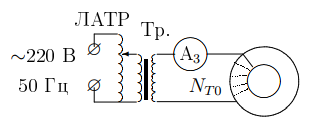
\includegraphics[height = 3cm, width = 7cm]{image3.png}
	\caption{Схема установки для размагничивания образца}
\end{figure}
\section*{Ход работы}
\subsection*{Предельная петля гистерезиса}
	Соберём схему согласно рис.1. Измерение петли начнём с максимального тока намагничивания. Будем отмечать величину тока $I$, соответствующую каждой позиции тумблера генератора, и отклонения зайчика $\Delta x$, соответствующие каждому щелчку. Измеряя шаг за шагом отклонения зайчика при изменениях тока, мы пройдём всю петлю гистерезиса. При движении по петле ток должен меняться строго монотонно. Если случайно пропущен один отброс зайчика, то мы не сможем вернуться назад на один шаг, так как это приведёт к искажению петли.	
\begin{table}[h!]
	\centering
	\begin{tabular}{|c|c|c|c|c|c|c|c|c|c|c|}
	\hline
		$I$, мА & 1469.6 & 538.1 & 243.8 & 146.5 & 96.0 & 64.5 & 49.0 & 39.6 & 33.7 & 30.8 \\
	\hline
		$\Delta x$, см & 10.3 & 10.6 & 7.5	& 5.6	& 4.5	& 2.6	& 1.7	& 1.1	& 0.6	 & 0.8 \\
	\hline	
	   $I$, mA & 26.9 & 23.4 &  0.41 \\	   
	\cline{1-4}
		$\Delta x$, см & 0.7	& 6.2	& 0.1  \\		  
	\cline{1-4}
	\end{tabular}
\end{table}
\newpage
\begin{table}[h!]
	\centering
	\begin{tabular}{|c|c|c|c|c|c|c|c|c|c|c|}
	\hline
		$I$, мА & 0.45 & 23.5 & 27.1 & 30.9 & 33.9 & 39.8 & 49.3 & 64.6 & 96.1 & 146.6 \\
	\hline
		$\Delta x$, см & 0.1 & 10.3 & 2.4	& 3.4	& 3.6	& 11.5	& 19.6	& 18.8	& 19.5	& 14.7\\
	\hline	
	   $I$, mA & 243.9 & 538.5 & 1472.4 \\	   
	\cline{1-4}
		$\Delta x$, см & 14 & 17.4 & 13.5\\		  
	\cline{1-4}
	\end{tabular}
\end{table}
\begin{table}[h!]
	\centering
	\begin{tabular}{|c|c|c|c|c|c|c|c|c|c|c|}
	\hline
		$I$, мА & 1471.3 & 538.3 & 244.0 & 146.5 & 96.0 & 64.6 & 49.2 & 39.6 & 33.8 & 30.8 \\
	\hline
		$\Delta x$, см & 10.1 & 10.4 & 7.5	& 5.5	& 4.4	& 2.5	& 1.7	& 1.1	& 0.6	& 0.8\\
	\hline	
	   $I$, mA & 27.0 & 23.4 & 0.43 \\	   
	\cline{1-4}
		$\Delta x$, см & 0.8	& 6.1	& 0.1\\		  
	\cline{1-4}
	\end{tabular}
\end{table}
\begin{table}[h!]
	\centering
	\begin{tabular}{|c|c|c|c|c|c|c|c|c|c|c|}
	\hline
		$I$, мА & 0.50 & 23.5 & 27.1 & 30.9 & 33.9 & 39.8 & 49.3 & 64.7 & 96.1 & 146.6 \\
	\hline
		$\Delta x$, см & 0.1 & 10.3 & 2.4 & 3.3 & 3.6 & 11.5 & 19.3 & 18.3 & 19.2 & 14.5\\
	\hline	
	   $I$, mA & 244.0 & 538.5 & 1472.5 \\	   
	\cline{1-4}
		$\Delta x$, см & 13.7 & 17	& 13.4\\		  
	\cline{1-4}
	\end{tabular}
\end{table}
\par
	Напряжённость магнитного поля $H$ в тороиде зависит от тока, текущего в намагничивающей обмотке, как
	\begin{equation}
		H = \frac{N_\text{T0}}{\pi D} \, I, \label{H}
	\end{equation}
где $D$ --- средний диаметр тора.	
\subsection*{Калибровка гальванометра}
\par
	При измерении предельной петли гистерезиса мы подобрали значение $R_M$ так, чтобы зайчик не зашкаливал ($R_M$ > $R_C$), где $R_C$ --- сопротивление соленоида. В данной экспериментальной установке
	\begin{table}[h!]
		\centering
		\begin{tabular}{|c|c|c|c|c|c|c|c|c|}
		\hline
			$R_M$, Ом & $R_C$, Ом & $l_C$, м & $d_C \, / \, d_T$ & $D$, м & $N_\text{C1}$, втк & $N_\text{C0}$, втк & $N_\text{T1}$, втк & $N_\text{T0}$, втк \\
		\hline
			100 & 60 & 0.8 & 7 & 0.1 & 435 & 825 & 300 & 1750 \\
		\hline	
		\end{tabular}
	\end{table}
\par
	Для калибровки гальванометра соберём схему согласно рис.2. Уменьшим на магазине сопротивление значение $R_M$ на величину $R_C$: $R_M' = R_M - R_C$. Установим тумблер генератора тока на максимум и, замкнув ключ $P_1$, запишем значение тока $I_\text{max}$. Подключив гальванометр и разомкнув ключ $P_1$, измерим отклонение гальванометра $\Delta x_1$, возникшее при изменении тока $\Delta I_1 = I_\text{max}$. В результате получим, что
	\begin{align*}
		\Delta x_1  &= \left(8.0 \pm 0.1\right) \, \text{см} \\
		\Delta I_1 &= \left(1472 \pm 1 \right) \, \text{мА} \\
		\frac{\Delta I_1}{\Delta x_1} &= \left(0.184 \pm 0.002\right) \, \frac{\text{А}}{\text{см}} \\
	\end{align*} 
\par
	Теперь мы сможем найти изменение магнитной индукции через отношение $\Delta I_1 / \Delta x_1$ и величину $\Delta x$:
	\begin{equation}
		\Delta B = \mu_0 {\left(\frac{d_C}{d_T}\right)}^2\, \frac{R}{R_1} \, \frac{N_\text{C0}}{N_\text{T1}} \, \frac{N_\text{C1}}{l_C} \, \frac{\Delta I_1}{\Delta x_1} \, \Delta x \label{B}
	\end{equation}
\subsection*{Начальная кривая намагничивания}
\par
	Начальную кривую намагничивания можно снять по той же схеме (рис.1), если предварительно размагнитить тороид в цепи переменного тока. Для этого соберём схему, изображённую на рис.3. Включим лабораторный автотрансформатор в сеть и установим ток, соответствующий насыщению. Ручкой лабораторного автотрансформатора медленно будем уменьшать ток до нуля. Затем вновь подсоедим тороид к цепи, изображённой на рис.1 и снимем начальную кривую намагничивания скачками увеличивая ток от нуля до $I_\text{max}$ 	
\begin{table}[h!]
	\centering
	\begin{tabular}{|c|c|c|c|c|c|c|c|c|c|c|}
	\hline
		$I$, мА & 0.39 & 23.97 & 27.63 & 31.43 & 34.42 & 40.47 & 50.01 & 65.25 & 96.72 & 147.25\\
	\hline
		$\Delta x$, см & 0.1 & 4.1 & 1.3 & 1.7 & 1.6 & 3.6 & 5.6 & 7.4 & 10.1 & 9.3\\
	\hline	
	   $I$, mA & 244.36 & 537.9 & 1470.2 \\	   
	\cline{1-4}
		$\Delta x$, см & 9.7 & 12.4 & 9.9\\		  
	\cline{1-4}
	\end{tabular}
\end{table}
\subsection*{Построение петли гистерезиса}
\par
	Построим петлю гистерезиса $B = f(H)$, используя формулы (\ref{B}) и (\ref{H}) для нахождения изменения магнитной индукции и напряжённости поля соответственно. Построение удобно начать с максимального значения $H$. Переход к следующему значению $H$ соответствует первому скачку $\Delta B$ и т.д. Отложив все $\Delta B$ по одной стороне петли и дойдя до насыщения, построим вторую сторону таким образом. Также построим начальную кривую намагничивания на этом же графике.
	\begin{figure}[h!]
		\centering
		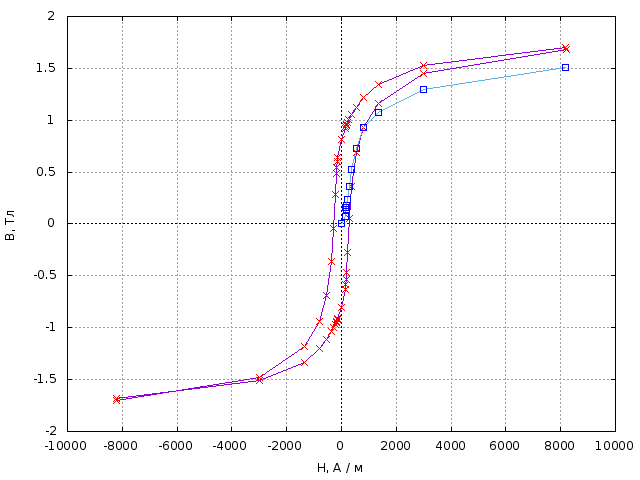
\includegraphics[height = 9cm, width = 16cm]{plot1.png}
		\caption{Предельная петля гистерезиса и начальная кривая намагничивания}
	\end{figure}
\subsection*{Исследование петли гистерезиса}
\par
	Определим по графику коэрцитивную силу $H_c$, индукцию насыщения $B_s$, а также определим максимальное значение дифференциальной магнитной проницаемости $\mu_\text{диф}$ для начальной кривой намагничивания. Проведя вычисления, получим, что
\begin{align*}
	H_c &= \left(274 \pm 2\right) \, \frac{\text{А}}{\text{м}} \\ 
	B_s &= \left(1.70 \pm 0.04\right) \, \text{Тл} \\
	\mu_\text{диф} &= \left(3504 \pm 175\right) \\
\end{align*}
\end{document}







